%=============================================================================
%  IEEE two-column report -- ECG telemetry and beat classification
%
%  OVERLEAF
%  1. New Project -> Upload Project -> upload this folder (report.tex +
%     figures/).
%  2. Menu -> Compiler -> pdfLaTeX.  Main document: report.tex.
%  3. Fill in the \author block below.
%  4. Search for "SCREENSHOT" -- each is a placeholder box for one of your own
%     images. Each says which assignment objective it covers.
%
%  The four data figures in figures/ are produced by tools/gen_figures.py from
%  the real pipeline, so they cannot drift away from the code.
%=============================================================================
\documentclass[conference]{IEEEtran}
\IEEEoverridecommandlockouts

\usepackage{cite}
\usepackage{amsmath,amssymb}
\usepackage{graphicx}
\usepackage{booktabs}
\usepackage{xcolor}
\usepackage{url}
\usepackage[hidelinks]{hyperref}
\usepackage{tikz}
\usetikzlibrary{arrows.meta,positioning,fit,backgrounds,calc}

\graphicspath{{figures/}}

\hyphenation{supra-ven-tricu-lar classi-fi-ca-tion re-sam-pling}

%-----------------------------------------------------------------------------
% Placeholder for a screenshot you still need to take. Replace the whole
% \screenshot{...} call with:
%     \includegraphics[width=\linewidth]{figures/your_image.png}
%-----------------------------------------------------------------------------
\newcommand{\screenshot}[2][0.55]{%
  \setlength{\fboxsep}{0pt}%
  \fcolorbox{gray!60}{gray!8}{%
    \parbox[c][#1\linewidth][c]{\linewidth}{%
      \centering\footnotesize\color{gray!80}%
      \textbf{[ SCREENSHOT ]}\\[2pt]#2}}}

%-----------------------------------------------------------------------------
\begin{document}

\title{An End-to-End ECG Monitoring System:\\
       Bluetooth Streaming, Mobile Display, and\\
       Automatic Heartbeat Classification}

\author{
\IEEEauthorblockN{Author Name}
\IEEEauthorblockA{\textit{Department of Electrical and Computer Engineering}\\
\textit{University Name}\\
City, Country \\
email@university.edu}
}

\maketitle

%-----------------------------------------------------------------------------
\begin{abstract}
This report describes a complete ECG monitoring system built from five parts. A
Raspberry Pi reads a recording from the PhysioNet MIT-BIH Arrhythmia Database,
resamples it to 250\,Hz, and sends it over Bluetooth to an Android phone. The
phone receives the signal and draws it on screen in real time. It then sends the
signal over Wi-Fi to a server, which finds each heartbeat, sorts it into normal
or abnormal, and sends the answer back. The same analysis was also written in
Java and run on the phone itself, so the system still works without a network.
Across 22 patients not used during development, heartbeat detection reached
98.0\% sensitivity and 99.8\% precision. A decision tree classifier reached
77.2\% overall accuracy and correctly identified 76.0\% of ventricular ectopic
beats. An automatic test confirms that the phone and the server produce
identical results from the same signal.
\end{abstract}

\begin{IEEEkeywords}
electrocardiography, QRS detection, Pan--Tompkins, arrhythmia classification,
Bluetooth, Android, mobile health
\end{IEEEkeywords}

%-----------------------------------------------------------------------------
\section{Introduction}

A long ECG recording contains far more heartbeats than a doctor can check by
hand. A single day of monitoring holds around 100{,}000 of them. Software that
finds the abnormal beats automatically is therefore essential if monitoring is
going to be useful outside a hospital.

This project builds the full chain such a system needs. The assignment set five
tasks, and this report follows them in order:

\begin{enumerate}
\item send an ECG signal at 250\,Hz over Bluetooth;
\item receive that signal on a phone;
\item draw the signal on the phone screen;
\item send the signal onward to a server over Wi-Fi;
\item run signal processing and a classifier on the server, and send the results
      back to the phone.
\end{enumerate}

An optional extra task was to run the signal processing and the classifier on
the phone instead of the server. This was also completed. Because the analysis
then exists twice, in Python and in Java, an automatic test was written to check
that the two versions agree exactly.

Section~\ref{sec:overview} gives an overview of the system. Sections
\ref{sec:part1} to \ref{sec:part5} cover the five tasks in turn.
Section~\ref{sec:bonus} covers the on-phone version, Section~\ref{sec:results}
gives the results, and Section~\ref{sec:limits} discusses what the system does
not do well.

%-----------------------------------------------------------------------------
\section{System Overview}
\label{sec:overview}

Fig.~\ref{fig:arch} shows how the parts fit together. A Raspberry Pi acts as the
sensor. An Android phone receives, displays and optionally analyses the signal. A
laptop acts as the server. All three sit on the same Wi-Fi network.

\begin{figure*}[!t]
\centering
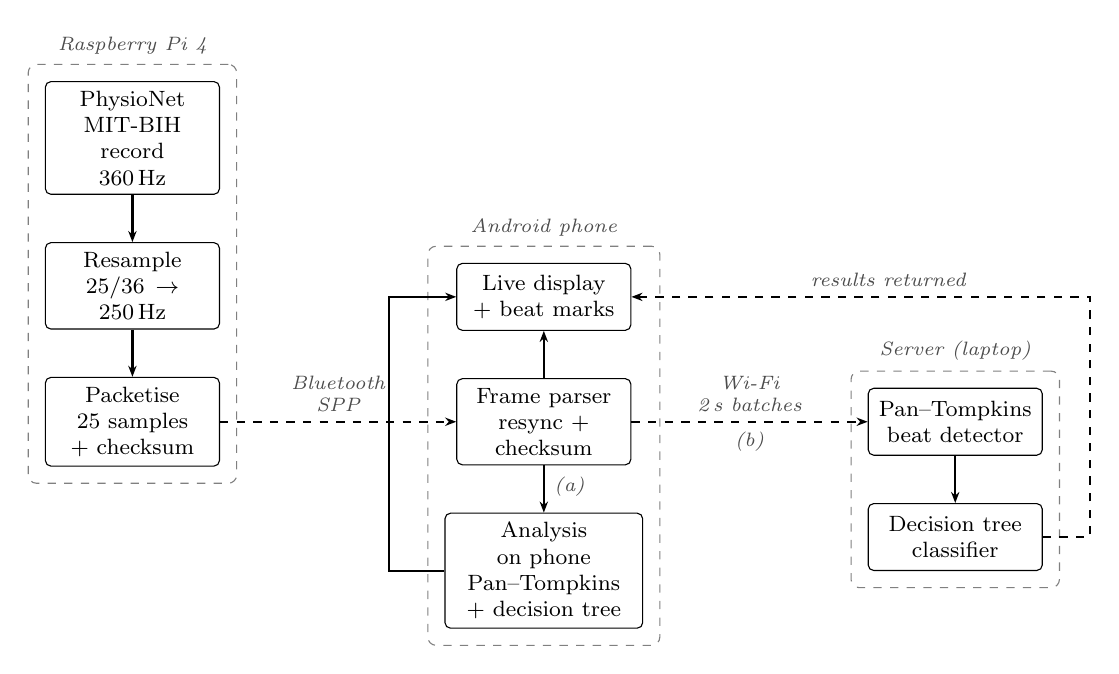
\begin{tikzpicture}[
  font=\footnotesize,
  box/.style={draw,rounded corners=2pt,align=center,minimum height=8.5mm,
              inner xsep=3pt,text width=20mm,fill=white},
  wide/.style={box,text width=23mm},
  flow/.style={-{Stealth[length=4pt]},thick},
  link/.style={-{Stealth[length=4pt]},thick,dashed},
  grp/.style={draw=gray,dashed,rounded corners=3pt,inner sep=6pt},
  lbl/.style={font=\scriptsize\itshape,text=gray!60!black},
]
% phone column (the anchor)
\node[box] (fp) {Frame parser\\resync + checksum};
\node[box,above=6mm of fp] (disp) {Live display\\+ beat marks};
\node[wide,below=6mm of fp] (ondev) {Analysis on phone\\Pan--Tompkins\\+ decision tree};
\draw[flow] (fp) -- (disp);
\draw[flow] (fp) -- node[lbl,right,pos=0.45]{(a)} (ondev);
\draw[flow] (ondev.west) -- ++(-7mm,0) |- (disp.west);

% Raspberry Pi
\node[box,left=30mm of fp] (pk) {Packetise\\25 samples\\+ checksum};
\node[box,above=6mm of pk] (rs) {Resample\\$25/36\rightarrow250$\,Hz};
\node[box,above=6mm of rs] (rec) {PhysioNet\\MIT-BIH record\\360\,Hz};
\draw[flow] (rec) -- (rs);
\draw[flow] (rs) -- (pk);

% server
\node[box,right=30mm of fp] (srv) {Pan--Tompkins\\beat detector};
\node[box,below=6mm of srv] (clf) {Decision tree\\classifier};
\draw[flow] (srv) -- (clf);

% links between devices
\draw[link] (pk) -- node[lbl,above,align=center]{Bluetooth\\SPP} (fp);
\draw[link] (fp.east) -- node[lbl,above,align=center]{Wi-Fi\\2\,s batches}
                        node[lbl,below,pos=0.5]{(b)} (srv.west);
\draw[link] (clf.east) -- ++(6mm,0) |- node[lbl,above,pos=0.72]{results returned} (disp.east);

\begin{scope}[on background layer]
  \node[grp,fit=(rec)(rs)(pk),label={[lbl]above:Raspberry Pi 4}] {};
  \node[grp,fit=(disp)(fp)(ondev),label={[lbl]above:Android phone}] {};
  \node[grp,fit=(srv)(clf),label={[lbl]above:Server (laptop)}] {};
\end{scope}
\end{tikzpicture}
\caption{The complete system. Solid arrows are processing steps inside one
device; dashed arrows are wireless links. The beat analysis exists twice and the
phone uses one path at a time: (a) everything runs on the phone and no network
is needed, or (b) the signal is sent to the server and the labels come back. The
two paths run identical algorithms, one written in Java and one in Python, and
an automatic test confirms they agree exactly.}
\label{fig:arch}
\end{figure*}

%-----------------------------------------------------------------------------
\section{Part 1: Sending the ECG over Bluetooth}
\label{sec:part1}

\subsection{Getting the signal}

Real ECG recordings were taken from the MIT-BIH Arrhythmia
Database~\cite{moody2001} on PhysioNet~\cite{goldberger2000}. Each recording
comes with labels written by cardiologists saying what type every heartbeat is.
Those labels are what make it possible to measure how well the classifier works.

The database is recorded at 360\,Hz, but the assignment asks for 250\,Hz. The
ratio $250/360$ simplifies to $25/36$, so the signal is resampled by a factor of
25 up and 36 down using a polyphase filter, which filters the signal before
throwing samples away.

It is worth being clear about why that filter matters, because the point is easy
to overstate. Without it, frequencies between 125\,Hz and 180\,Hz fold down into
the 70--125\,Hz range, so a 150\,Hz muscle artefact would reappear as a false
100\,Hz signal, as Fig.~\ref{fig:resample} shows. This folding cannot reach the
5--15\,Hz band used to find heartbeats, because that would need energy at
235--245\,Hz, which a 360\,Hz recording cannot contain. Beat detection is
therefore safe either way. What the filter protects is the shape of the waveform
shown on screen.

\begin{figure}[!t]
\centering
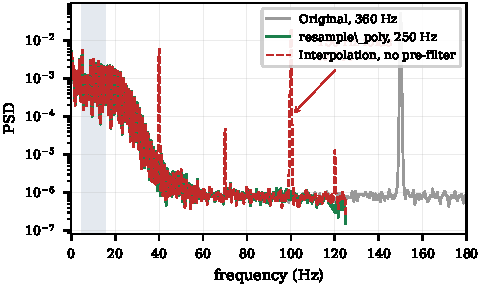
\includegraphics[width=\linewidth]{fig_resample.pdf}
\caption{Frequency content before and after resampling from 360\,Hz to 250\,Hz.
Without a filter a 150\,Hz component reappears at 100\,Hz. The shaded band is
where the beat detector works.}
\label{fig:resample}
\end{figure}

\subsection{The packet format}

Bluetooth Serial Port Profile sends a plain stream of bytes with no markers
showing where one message ends and the next begins, so the program adds its own
structure:

\begin{center}\footnotesize\ttfamily
0xA5 0x5A | seq | count | 25 samples | checksum
\end{center}

Each packet holds 25 samples, which is 100\,ms of signal, so ten packets are
sent every second. Sending one sample per packet would waste more space on
headers than on the data itself.

Three things can go wrong on a wireless link: the phone can connect halfway
through a packet, a byte can be corrupted, and data arrives in chunks of random
size. The receiver handles all three by searching for the two marker bytes,
checking the checksum, and moving forward one byte at a time whenever something
does not match. This loses one packet instead of the whole connection.

One detail proved important during testing. The receiver must check that the
length byte is sensible \emph{before} using it. A corrupted length claiming that
512 samples follow made the receiver wait forever for bytes that would never
arrive, freezing the link permanently rather than losing a single packet.

%-----------------------------------------------------------------------------
\section{Parts 2 and 3: Receiving and Displaying on the Phone}
\label{sec:part23}

The Android app connects to the Raspberry Pi over Bluetooth and reads the byte
stream. Reading, decoding and filtering all happen on a background thread. Only
short text updates are sent to the screen thread, so the display stays smooth
while data arrives continuously.

The waveform is drawn the way a hospital monitor draws it. New samples are
written into a circular buffer and a small gap is cleared just ahead of the
writing position, which gives a sweeping trace. The simpler approach of shifting
the whole array left on every frame was avoided because it copies the entire
buffer every frame and makes the trace flicker.

The screen is redrawn about 30 times per second rather than every time a packet
arrives. The display cannot show more than this, and redrawing more often only
wastes battery. Where the screen size allows, the grid follows the standard ECG
paper scale of 25\,mm/s and 10\,mm/mV, so the trace looks familiar.

\begin{figure}[!t]
\centering
\screenshot[0.95]{%
  \textbf{Live ECG on the phone}\\[4pt]
  Objectives 2 and 3.\\[3pt]
  Take this while the app is streaming. Make sure the heart
  rate, the moving trace and at least one coloured beat
  marker are all visible.}
\caption{The app showing a live ECG. Marks above the trace are coloured by beat
type: green for normal, amber for supraventricular, red for ventricular.}
\label{fig:app}
\end{figure}

%-----------------------------------------------------------------------------
\section{Part 4: Sending the Signal to the Server}
\label{sec:part4}

The phone collects two seconds of signal (500 samples) before sending anything.
Sending each 25-sample packet immediately would mean ten network requests every
second, and each request carries more header information than actual data, so
the battery cost would be high.

The waiting queue has a fixed size. If the network cannot keep up, the oldest
batch is thrown away rather than stored. For a live monitor old ECG data is of
little use, and a queue with no limit simply grows until the phone runs out of
memory and closes the app.

%-----------------------------------------------------------------------------
\section{Part 5: Server Processing and Classification}
\label{sec:part5}

\subsection{Finding the heartbeats}

Heartbeats are found using the Pan--Tompkins method~\cite{pan1985}, written to
process one sample at a time so it can run on a live stream. The stages are
shown in Fig.~\ref{fig:pipeline}:

\begin{enumerate}
\item a 5--15\,Hz bandpass filter, which keeps the sharp part of the heartbeat
      and removes baseline drift and muscle noise;
\item a derivative, which responds to how steeply the signal rises;
\item squaring, which makes everything positive and exaggerates large slopes;
\item a 150\,ms moving average, which turns each beat into a single smooth bump.
\end{enumerate}

Bumps are then accepted as heartbeats using thresholds that adapt to the signal,
with a 200\,ms blocking period so one beat cannot be counted twice, and a check
that rejects T~waves by comparing how steeply they rise.

\begin{figure}[!t]
\centering
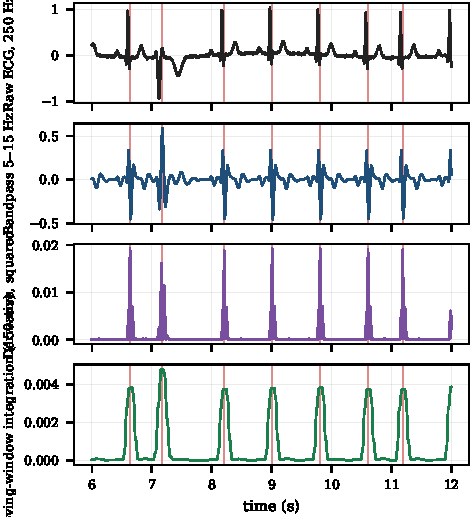
\includegraphics[width=\linewidth]{fig_pipeline.pdf}
\caption{The four stages of the beat detector over six seconds of ECG. Vertical
lines mark where beats were found. Each stage makes the heartbeat stand out more
clearly from everything else.}
\label{fig:pipeline}
\end{figure}

\subsection{Locating the exact beat position}

Finding the exact position of each beat mattered more than expected, because
every shape measurement is taken relative to it.

The first version searched nearby for the largest point of the filtered signal.
This failed because a filtered heartbeat swings both up and down, so the search
landed on the upward peak for one beat and the downward peak for the next.

The second version searched for whichever position best matched the patient's
own normal beat. This was worse, and in a way that was hard to see. Because it
kept the best possible match, the similarity score became a best case rather than
a fair measurement. On record 233, beats that cardiologists had marked as
ventricular scored between 0.83 and 0.98 similarity against the patient's normal
beat. The test for ``different shape'' therefore never triggered, and two-thirds
of abnormal beats were missed.

The final version uses the centre of energy of the beat,
\begin{equation}
c = \frac{\sum_k f^2[k]\,k}{\sum_k f^2[k]},
\label{eq:centroid}
\end{equation}
where $f[k]$ is the filtered signal. This is a plain physical definition, the
middle of the beat, which means the same thing for a narrow normal beat and a
wide abnormal one. It does not look at the template at all, so the similarity
score measured afterwards is honest.

\subsection{Describing each beat}

Nine measurements are taken for every beat, listed in Table~\ref{tab:features}.
They are written as \emph{ratios} against the patient's own normal beats rather
than as fixed numbers of millivolts or milliseconds. Fixed limits do not transfer
between patients or between electrode positions; ratios largely do.

\begin{table}[!t]
\caption{Measurements taken for each heartbeat}
\label{tab:features}
\centering
\footnotesize
\begin{tabular}{@{}lll@{}}
\toprule
\textbf{Name} & \textbf{Meaning} & \textbf{Tells us} \\
\midrule
\texttt{rr\_prev}        & gap before the beat (s) & heart rate \\
\texttt{rr\_next}        & gap after the beat (s)  & pause length \\
\texttt{rr\_ratio}       & gap before / average    & how early \\
\texttt{rr\_next\_ratio} & gap after / average     & pause after \\
\texttt{width\_ratio}    & width / normal width    & how wide \\
\texttt{amp\_ratio}      & height / normal height  & signal quality \\
\texttt{corr}            & similarity to normal    & shape \\
\texttt{rr\_asym}        & change in gap           & rhythm pattern \\
\texttt{area\_ratio}     & area / normal area      & size of the beat \\
\bottomrule
\end{tabular}
\end{table}

Each beat is classified one beat late, so that the gap \emph{after} it is known.
This delay is deliberate. The standard way to tell a ventricular beat from an
atrial one is the pause that follows it. A ventricular beat does not reset the
heart's natural pacemaker, so the next normal beat arrives on schedule and the
pause is long. An atrial beat does reset it, so the pause is shorter.

Fig.~\ref{fig:features} shows how well these measurements separate the beat types
on real data.

\begin{figure*}[!t]
\centering
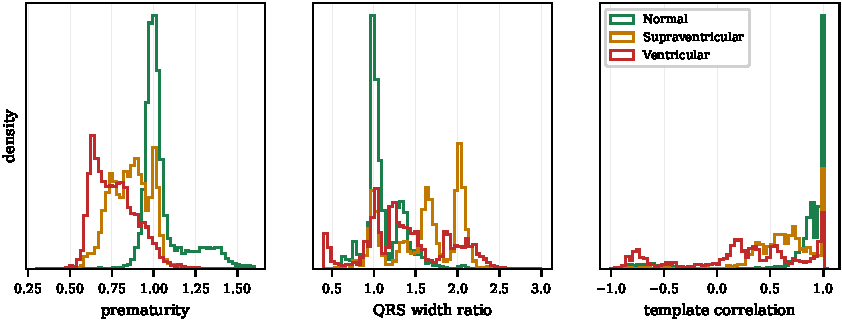
\includegraphics[width=\textwidth]{fig_features.pdf}
\caption{How three of the measurements separate the beat types, using 22{,}781
real heartbeats from MIT-BIH with cardiologist labels. Ventricular beats are
earlier, wider and less similar in shape. The overlap between the curves is why
no single measurement is enough on its own.}
\label{fig:features}
\end{figure*}

\subsection{Choosing the classifier}

Two classifiers were compared. The first uses fixed rules written by hand from
textbook criteria and needs no training data. The second is a decision tree
fitted to the labelled data.

Fixed rules turned out to be hard to set correctly. Thresholds were first chosen
using a synthetic test signal, and twice they behaved differently on real
recordings. In one case a threshold was set from the list of wrongly classified
beats, which are by definition the unusual ones, and the conclusion drawn from
them did not hold for the rest of the data. Fitting the thresholds to the data
avoided this.

A decision tree of depth 3 was chosen. Deeper trees scored \emph{worse} on
patients they had not seen, because they began learning the habits of individual
patients rather than general rules. A shallow tree is also small enough to copy
onto the phone as a few comparisons, and simple enough to read, so the rules it
learned can be checked against medical expectation. Those rules were sensible: it
splits first on how early the beat is, then uses \emph{how much} earlier to
separate ventricular from atrial beats, and falls back on shape for beats that
are not early.

Logistic regression was also tried and performed noticeably worse
(Table~\ref{tab:classifiers}), which suggests the boundary between beat types is
not a straight line in these measurements.

\begin{figure}[!t]
\centering
\fbox{\parbox{0.92\linewidth}{\footnotesize\raggedright
\hspace*{0em}if how early (gap before / average) $\leq$ 0.895:\\
\hspace*{2em}if gap before beat (s) $\leq$ 0.638:\\
\hspace*{4em}if QRS width (s) $\leq$ 0.053:\\
\hspace*{6em}\textbf{Ventricular} (68\% confident)\\
\hspace*{4em}else:\\
\hspace*{6em}\textbf{Ventricular} (97\% confident)\\
\hspace*{2em}else:\\
\hspace*{4em}if gap before beat (s) $\leq$ 0.792:\\
\hspace*{6em}\textbf{Supraventricular} (89\% confident)\\
\hspace*{4em}else:\\
\hspace*{6em}\textbf{Normal} (95\% confident)\\
\hspace*{0em}else:\\
\hspace*{2em}if QRS width / normal width $\leq$ 1.594:\\
\hspace*{4em}if area / normal area $\leq$ 1.729:\\
\hspace*{6em}\textbf{Normal} (96\% confident)\\
\hspace*{4em}else:\\
\hspace*{6em}\textbf{Ventricular} (49\% confident)\\
\hspace*{2em}else:\\
\hspace*{4em}if shape similarity to normal $\leq$ 0.258:\\
\hspace*{6em}\textbf{Ventricular} (89\% confident)\\
\hspace*{4em}else:\\
\hspace*{6em}\textbf{Normal} (53\% confident)\\
}}
\caption{The decision tree learned from the training patients. Its depth is capped at 3 so that it stays readable and can be checked against clinical expectation: it splits first on how early the beat is, then on how much earlier, and falls back on shape for beats that are not early.}
\label{fig:tree}
\end{figure}

%-----------------------------------------------------------------------------
\section{Optional Task: Running Everything on the Phone}
\label{sec:bonus}

The detector and the classifier were rewritten in Java and run on the phone. The
cost is about 40 arithmetic operations per sample, which at 250\,Hz is far below
what any modern phone can do. With this enabled the phone needs no network at
all.

Keeping the same method written twice, once in Python and once in Java, creates
an obvious risk: the two could quietly drift apart and give different answers for
the same patient. An automatic test was therefore written. It compiles the
phone's code with a normal Java compiler, runs both versions over the same
signal, and compares every beat position, every measurement and every label. It
reports agreement to six decimal places, and it is run after any change to either
version.

\begin{figure}[!t]
\centering
\screenshot[0.42]{%
  \textbf{Agreement test output}\\[4pt]
  Terminal output of \texttt{cross\_check.py} showing
  \texttt{MATCH}. This is the evidence that the phone and
  the server give the same answers.}
\caption{Output of the automatic test comparing the Python and Java versions of
the analysis.}
\label{fig:crosscheck}
\end{figure}

%-----------------------------------------------------------------------------
\section{Results}
\label{sec:results}

\subsection{The wireless link}

The packet decoder was tested against the three failure types described in
Section~\ref{sec:part1}. Results are in Table~\ref{tab:link}. The output was
identical no matter how the data was broken into chunks, and any single corrupted
byte cost exactly one packet.

\begin{table}[!t]
\caption{Behaviour of the packet decoder under faults}
\label{tab:link}
\centering
\footnotesize
\begin{tabular}{@{}ll@{}}
\toprule
\textbf{Test} & \textbf{Result} \\
\midrule
Chunks of 1, 7, 56, 4096 bytes & identical output every time \\
Corrupted marker bytes         & 1 packet lost, then recovered \\
Corrupted length byte          & 1 packet lost, then recovered \\
Corrupted data or checksum     & 1 packet lost, then recovered \\
Joining partway through        & recovered at the next packet \\
\bottomrule
\end{tabular}
\end{table}

A full test streaming 12 seconds of ECG from the transmitter to the receiving
code delivered 120 packets and 3000 samples with nothing lost, which is exactly
the expected rate of 250 samples per second.

\subsection{Finding heartbeats}

Beat detection was measured on 22 recordings that were not used during
development, following the standard patient split of de~Chazal
\emph{et al.}~\cite{dechazal2004}. A beat counted as found if it lay within
150\,ms of a cardiologist's mark.

\begin{table}[!t]
\caption{Beat detection on 22 unseen patients}
\label{tab:detection}
\centering
\footnotesize
\begin{tabular}{@{}lr@{}}
\toprule
Beats marked by cardiologists & 49{,}712 \\
Beats found by the detector   & 48{,}834 \\
Correctly matched             & 48{,}740 \\
\midrule
\textbf{Sensitivity} (beats found)              & \textbf{98.04\%} \\
\textbf{Precision} (found beats that were real) & \textbf{99.81\%} \\
\bottomrule
\end{tabular}
\end{table}

Nearly all recordings were close to perfect. The exception was record 228, where
only about half the beats were found. That recording is known for heavy noise and
a wandering baseline, and the system has no check for poor signal quality.

\subsection{Classifying heartbeats}

The classifiers were compared on 22{,}781 labelled beats from ten recordings
using leave-one-record-out testing. Every recording is tested with a classifier
trained only on the other nine, so no classifier is ever tested on a patient it
has already seen.

\begin{table}[!t]
\caption{Classifier comparison, 22{,}781 beats, patient-disjoint testing}
\label{tab:classifiers}
\centering
\footnotesize
\begin{tabular}{@{}lccc@{}}
\toprule
& \textbf{Fixed rules} & \textbf{Logistic} & \textbf{Tree} \\
\midrule
Overall accuracy        & 72.2\% & 63.4\% & \textbf{77.2\%} \\
\midrule
Normal, found           & 78.3\% & 73.1\% & \textbf{87.6\%} \\
Normal, correct         & \textbf{95.8\%} & 90.7\% & 86.5\% \\
\midrule
Ventricular, found      & \textbf{80.1\%} & 46.0\% & 76.0\% \\
Ventricular, correct    & 39.0\% & 37.1\% & \textbf{67.3\%} \\
\midrule
Supraventricular, found & \textbf{15.0\%} & 8.7\% & 2.3\% \\
\bottomrule
\end{tabular}
\end{table}

The decision tree is the best overall. The most useful difference is how often it
is right when it reports a ventricular beat: 67.3\%, against 39.0\% for the fixed
rules. A monitor that raises a false alarm two times out of three is one that
staff will start to ignore, so this matters more than the headline accuracy
figure. Table~\ref{tab:confusion} gives the tree's results in full.

\begin{table}[!t]
\caption{Decision tree results in detail (rows are the true type)}
\label{tab:confusion}
\centering
\footnotesize
\begin{tabular}{@{}lrrrr@{}}
\toprule
& \textbf{Normal} & \textbf{Supra.} & \textbf{Vent.} & \textbf{Other} \\
\midrule
Normal           & 14{,}572 & 1{,}342 & 685 & 32 \\
Supraventricular & 1{,}068  & 43      & 725 & 6 \\
Ventricular      & 870      & 71      & \textbf{2{,}981} & 0 \\
Other            & 345      & 1       & 40  & 0 \\
\bottomrule
\end{tabular}
\end{table}

\subsection{Speed}

The server analysed a two-second batch of ECG in about 1.8\,ms on average. That
is roughly a thousand times faster than real time, so one server could handle a
large number of phones at once. On the phone the cost per sample is small enough
that the app stayed responsive throughout.

\begin{figure}[!t]
\centering
\screenshot[0.62]{%
  \textbf{Server dashboard}\\[4pt]
  Objectives 4 and 5.\\[3pt]
  Screenshot of the web page at
  \texttt{http://<server-ip>:8000/} while the phone is
  streaming, showing the trace and the beat table.}
\caption{The server dashboard receiving live data from the phone and showing the
classified beats being sent back.}
\label{fig:dashboard}
\end{figure}

\begin{figure}[!t]
\centering
\screenshot[0.62]{%
  \textbf{Hardware setup}\\[4pt]
  Objective 1.\\[3pt]
  Photograph of the Raspberry Pi next to the phone showing
  the live trace.}
\caption{The test setup. The Raspberry Pi stands in for a wearable sensor by
streaming a recorded ECG over Bluetooth.}
\label{fig:hardware}
\end{figure}

%-----------------------------------------------------------------------------
\section{Limitations}
\label{sec:limits}

\textbf{Supraventricular beats are not detected well.} Only 2.3\% are found.
These beats travel the normal path through the heart, so they look almost
identical to normal beats. The real clue is the P~wave in front of them, and none
of the measurements in this system look at the P~wave. This is an honest limit of
the chosen measurements, not a tuning problem.

\textbf{There is no signal quality check.} If an electrode comes loose the
detector will happily find ``beats'' in the resulting noise. Record 228 shows
this clearly. A real device would need to detect poor contact and stop reporting.

\textbf{The signal is a recording, not a live patient.} The system has never
faced movement artefacts, sweat, or a loose electrode, which are usually the main
sources of error in real monitoring.

\textbf{The ``Other'' group performs poorly.} It mixes fusion beats, paced beats
and unclassifiable ones together, and none of them are identified.

\textbf{This is not a medical device.} It was tested on a database, not validated
clinically, and must not be used to make decisions about anyone's health.

%-----------------------------------------------------------------------------
\section{Conclusion}

All five parts of the assignment were completed, along with the optional task of
running the analysis on the phone. The system reads a real ECG, sends it over
Bluetooth, displays it live, forwards it over Wi-Fi, and classifies each beat
either on the server or on the phone. Beat detection reached 98.0\% sensitivity
and 99.8\% precision on 22 unseen patients, and the decision tree classifier
reached 77.2\% accuracy with 76.0\% of ventricular beats correctly found.

The most useful lesson was about testing. Every serious problem in this
project---the frozen link caused by a bad length byte, the similarity score that
flattered abnormal beats, and thresholds that suited a synthetic test signal but
not real patients---was found by measuring, not by reading the code. Two of them
looked perfectly correct until real data disagreed. The automatic test comparing
the phone and server versions exists for exactly that reason.

%-----------------------------------------------------------------------------
\section*{Acknowledgment}

The authors thank the PhysioNet project for providing free access to the MIT-BIH
Arrhythmia Database.

%-----------------------------------------------------------------------------
\begin{thebibliography}{9}

\bibitem{pan1985}
J.~Pan and W.~J. Tompkins, ``A real-time QRS detection algorithm,''
\emph{IEEE Trans. Biomed. Eng.}, vol.~BME-32, no.~3, pp.~230--236, Mar. 1985.

\bibitem{moody2001}
G.~B. Moody and R.~G. Mark, ``The impact of the MIT-BIH Arrhythmia Database,''
\emph{IEEE Eng. Med. Biol. Mag.}, vol.~20, no.~3, pp.~45--50, May 2001.

\bibitem{goldberger2000}
A.~L. Goldberger \emph{et al.}, ``PhysioBank, PhysioToolkit, and PhysioNet:
Components of a new research resource for complex physiologic signals,''
\emph{Circulation}, vol.~101, no.~23, pp.~e215--e220, 2000.

\bibitem{dechazal2004}
P.~de~Chazal, M.~O'Dwyer, and R.~B. Reilly, ``Automatic classification of
heartbeats using ECG morphology and heartbeat interval features,''
\emph{IEEE Trans. Biomed. Eng.}, vol.~51, no.~7, pp.~1196--1206, Jul. 2004.

\bibitem{aami2012}
\emph{Testing and Reporting Performance Results of Cardiac Rhythm and ST Segment
Measurement Algorithms}, ANSI/AAMI Standard EC57, 2012.

\bibitem{luz2016}
E.~J.~S. Luz, W.~R. Schwartz, G.~C\'amara-Ch\'avez, and D.~Menotti, ``ECG-based
heartbeat classification for arrhythmia detection: A survey,''
\emph{Comput. Methods Programs Biomed.}, vol.~127, pp.~144--164, Apr. 2016.

\end{thebibliography}

\end{document}
